%%% Bibliography (literature used as a source)
%%%
%%% We employ biblatex to construct the bibliography. It processes
%%% citations in the text (e.g., the \cite{...} macro) and looks up
%%% relevant entries in the bibliography.bib file.
%%%
%%% See also biblatex settings in thesis.tex.

%%% Generate the bibliography. Beware that if you cited no works,
%%% the empty list will be omitted completely.

% We let bibliography items stick out of the right margin a little
\def\bibfont{\hfuzz=2pt}

%\printbibliography[heading=bibintoc]


%%%%

%\begin{document}

%\maketitle

\section{First section}


Let's cite! The Einstein's journal paper \cite{Student08}

\medskip

\begin{figure}
    \centering
    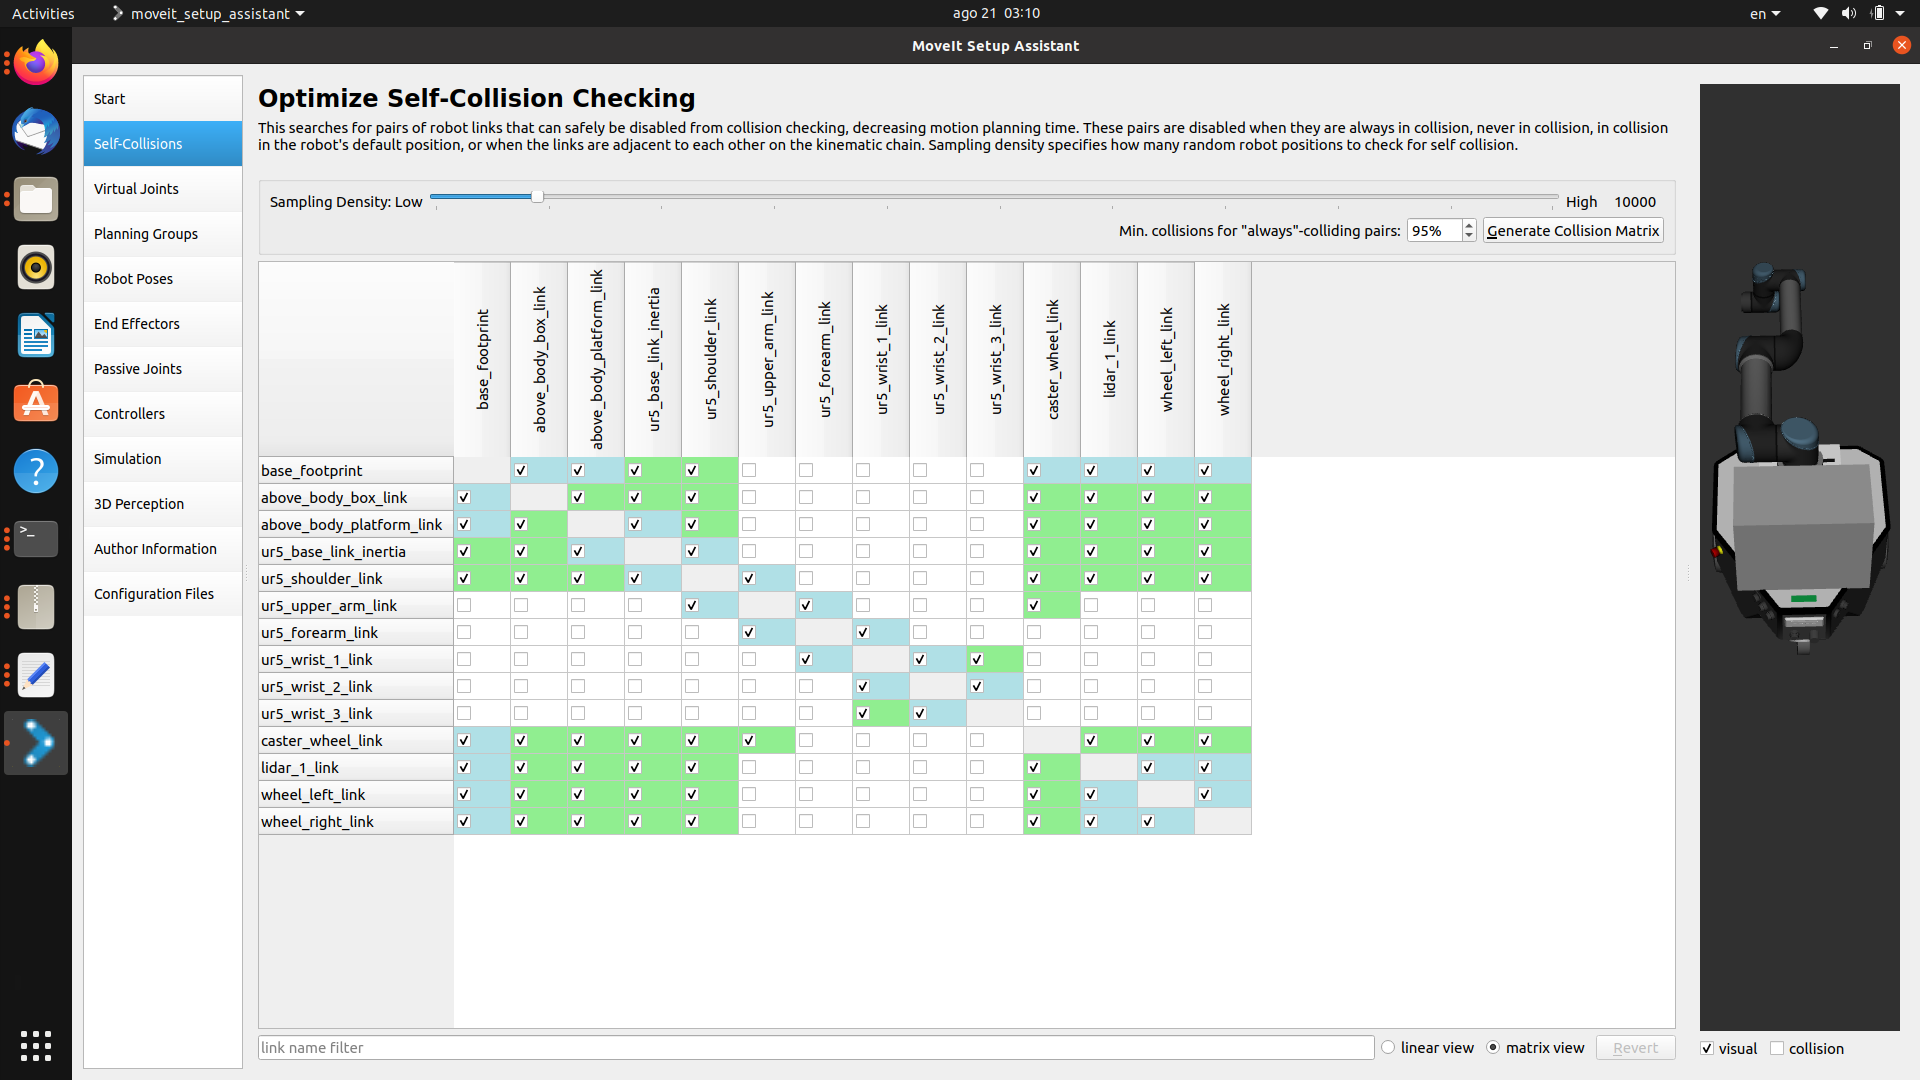
\includegraphics[width=0.5\linewidth]{SelfCollisionsMatrix.png}
    \caption{Enter Caption}
    \label{fig:enter-label}
\end{figure}

\printbibliography

%%%%
%%% If case you prefer to write the bibliography manually (without biblatex),
%%% you can use the following. Please follow the ISO 690 standard and
%%% citation conventions of your field of research.

% \begin{thebibliography}{99}
%
% \bibitem{lamport94}
%   {\sc Lamport,} Leslie.
%   \emph{\LaTeX: A Document Preparation System}.
%   2nd edition.
%   Massachusetts: Addison Wesley, 1994.
%   ISBN 0-201-52983-1.
%
% \end{thebibliography}
